\begin{figure}[h!]
\centering
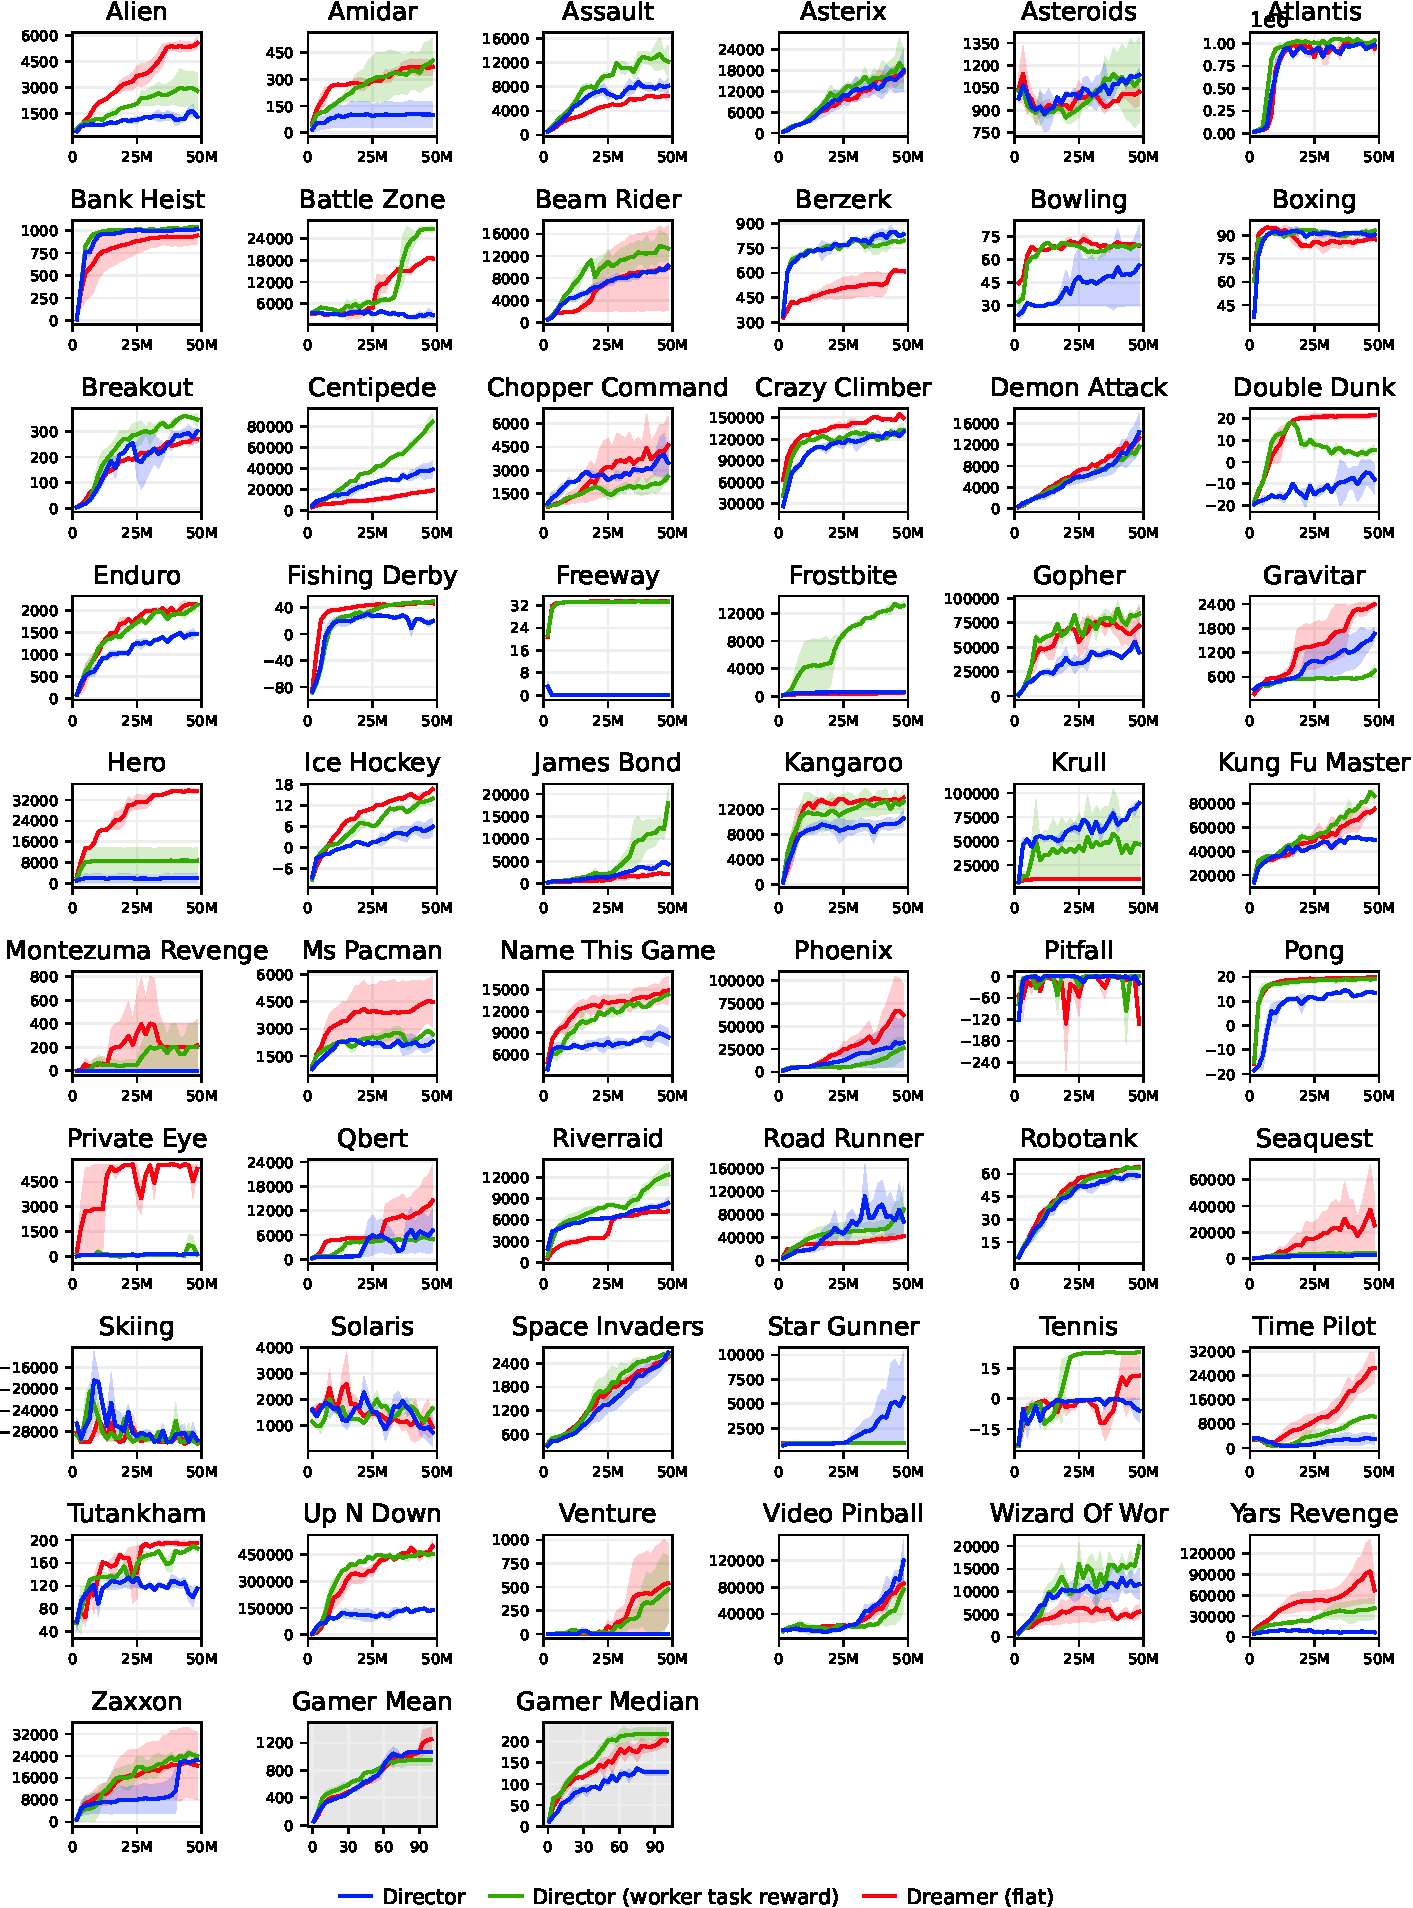
\includegraphics[width=0.97\textwidth]{atari/atari}
\caption{
To test the generality of Director, we evaluate it on 55 Atari games \citep{bellemare2013ale}. 
We find that Director solves a wide range of tasks despite giving no task reward to the worker.
Director is the first approach in the literature that demonstrates a hierarchy with task-agnostic worker performing reliably across many tasks. 
When additionally providing task reward to the worker, performance reaches that of Dreamer and even exceeds its human-normalized median score.
These experiments use no action repeat and train every 16 environment steps, resulting in faster wall clock time and lower sample efficiency than the results reported by \citet{hafner2019dreamer}.
}
\label{fig:atari}
\end{figure}
